\documentclass[a4paper,runningheads]{llncs}
\usepackage[T1]{fontenc}
\usepackage[table]{xcolor}
\usepackage{pgfplots}
\usepackage{amsmath,amssymb}
\usepackage{tikz}
\usetikzlibrary{shapes,shapes.geometric,arrows,fit,calc,positioning,automata,chains,matrix.skeleton, arrows.meta}
\tikzset{nature/.style={draw,rectangle}}
\tikzset{>={Stealth[scale=1.2]}}

\begin{document}

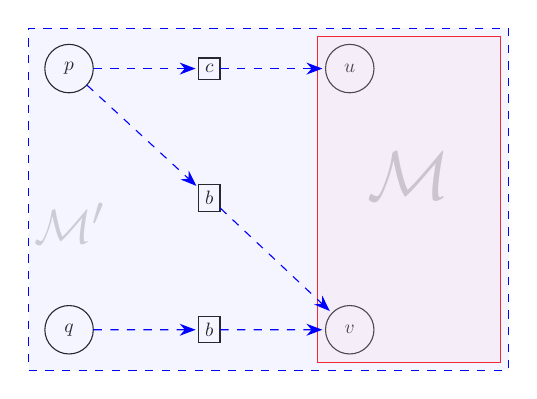
\begin{tikzpicture}[shorten >=1pt,auto,node distance=1.9 cm, scale = 0.7, transform shape]
    
        \node[state](p){$p$};
        \node[nature](pc)[right=of p]{$c$};
        \node[nature](pb)[below=of pc]{$b$};
        \node[nature](qb)[below=of pb]{$b$};
        \node[state](q)[left=of qb]{$q$};
        \node[state](u)[right=of pc]{$u$};
        \node[state](v)[right=of qb]{$v$};
        \node[](inv1)[right=of u]{};
        \node[](inv2)[right=of v]{};
        \node[](m')[above=1cm of q, text opacity=0.2]{\Huge{$\mathcal{M'}$}};
        \node       (X)    [draw=red, fit= (inv1) (v) (u), inner sep=0.1cm, fill=red!20, fill opacity=0.2] {\Huge{$\mathcal{M}$}};
        
        \node (Y) [draw=blue, fit= (inv1) (q) (p), inner sep=0.2cm, fill=blue!20, fill opacity=0.2, dashed] {};
        
        \path[->,color=blue,dashed] 
        (p)   edge [above] node [align=center] {} (pc)
              edge [above] node [align=center] {} (pb)
        (pc)  edge [above] node [align=center] {} (u)
        (pb)  edge [above] node [align=center] {} (v)
        (q)   edge [above] node [align=center] {} (qb)
        (qb)  edge [above] node [align=center] {} (v)
        ;
    \end{tikzpicture}

\end{document}